\section{LSM9DS1}\label{sec_design_LSM9DS1}
\textit{I dette afsnit designes, implementeres og testes accelerometeret og gyroskopet som benyttes til dataopsamling af aktiviteter.}

\subsection{Design} \label{design_lsm}
Der benyttes et integrated circuit (IC) af typen LSM9DS1, der kræver 3,3~V for at være optimal funktionel. Denne indeholder magnometer, gyroskop og accelerometer, hvoraf magnometeret ikke vil blive benyttet.\fxnote{Magnometeret benyttes til måling af givne paramtere på et magnetfelt} \\ 
Arbejdsområderne for accelerometeret og gyroskopet er valgbart, hvoraf det er muligt at indstille accelerometeret til $\pm$1, $\pm$4, $\pm$8 eller $\pm$16~g, og gyroskopet kan indstilles til $\pm$245, $\pm$500 eller $\pm$2000~dps. \citep{Jimb02016,STMicroelectronics2016} \\
På baggrund af kravene opstillet i \secref{Sec:krav}, vælges accelerometerets arbejdsområde til $\pm$16~g og gyroskopets arbejdsområde til $\pm$2000~dps. 

LSM9DS1 har seks frihedsgrader, når magnometeret fravælges, hvilket betyder, at den måler i x-, y- og z-aksen for accelerometeret og gyroskopet, som kan ses på \figref{vores_IC}. %Akserne for gyroskopet og accelerometeret internt følger højrehåndsreglen.
\citep{STMicroelectronics2016}\newline 
\begin{figure}[H]
	\centering
	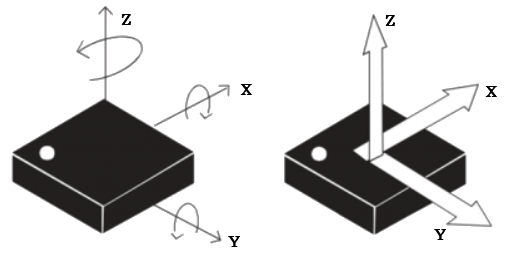
\includegraphics[scale=0.4]{figures/cDesign/LSM9DS1.png}
	\caption{Figuren viser akserne på LSM9DS1 for gyroskopet (venstre) og accelerometeret (højre). \citep{Jimb02016} (Modificeret)}
	\label{vores_IC}
\end{figure}

Sensorens opbygning fremgår af \figref{fig:IC_pins}, hvor der henholdsvis er fire pins på venstre side og 9 pins på højre side. ICens pins på højre side vil ikke blive benyttet.\\
De fire pins på venstre side af ICen vil blive benyttet til spændingstilkobling samt til at læse sensorens outputdata fra. GND og VDD er pins til henholdsvis jord og spændingsforsyning, mens SDA er I$^2$C datapin, hvor data bliver sendt og modtaget. SCL er en seriel clock, der blandt andet sørger for synkron dataopsamling.
\begin{figure}[H]
	\centering
	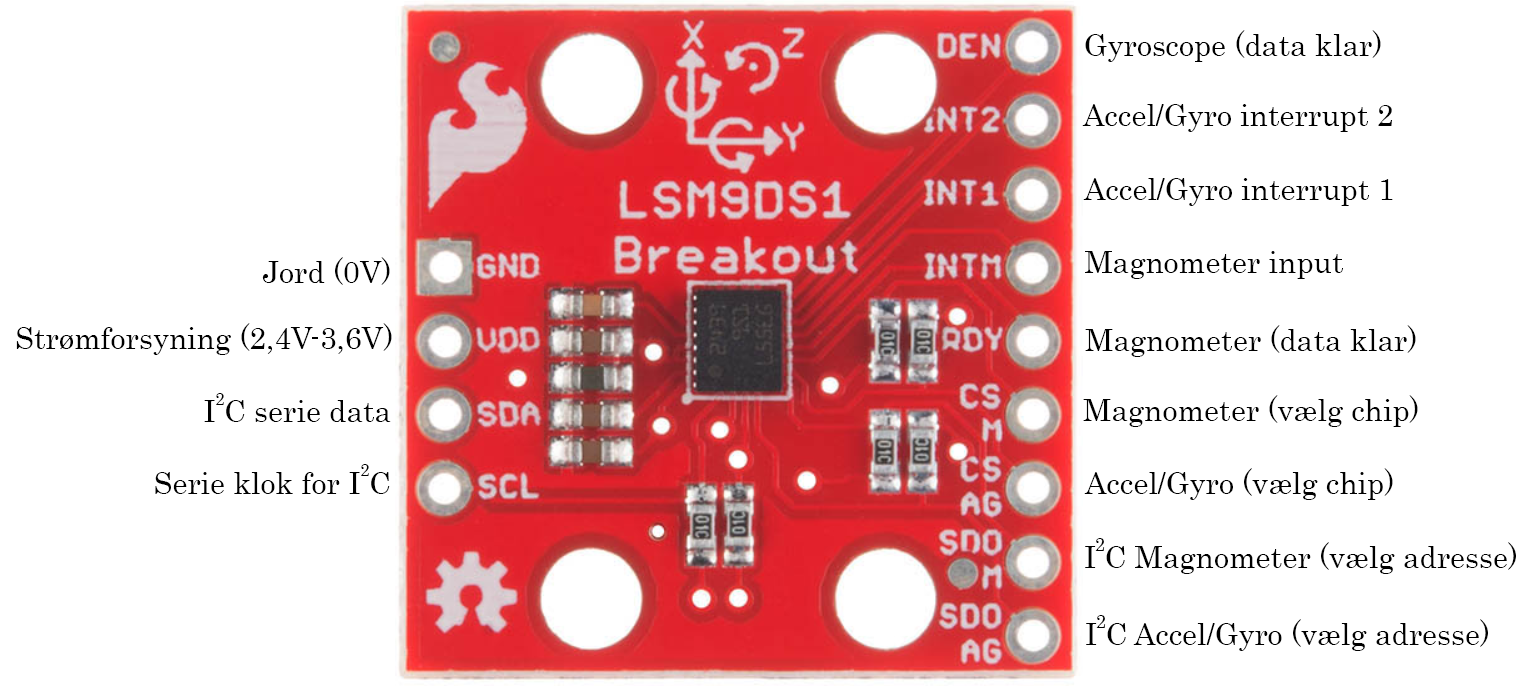
\includegraphics[scale=0.3]{figures/cDesign/accelerometeret.png}
	\caption{Figuren viser pinkonfigurationen af LSM9DS1. \citep{Jimb02016} (Modificeret)}
	\label{fig:IC_pins}
\end{figure}

LSM9DS1 er en digital sensor, hvormed de analoge signaler konverteres til digitale i ICen ved hjælp af en indbygget 16 bits ADC. Derfor skal sensoren konfigureres til en given samplingsfrekvens for ADCen. Ifølge \secref{krav_adc} skal accelerometret sample med mindst 450~Hz. Det fremgår af databladet for ICen, at accelerometret kan konfigureres til seks forskellige samplingsfrekvenser, hvoraf en samplingsfrekvens på 476~Hz har mindst afvigelse til den ønskede samplingsfrekvens. \\
Gyroskopet skal samples med mindst 60~Hz, men ifølge gyroskopets datablad kan den indstilles til 59,5~Hz eller 119~Hz, hvorfor samplingsfrekvensen vælges til 119~Hz.

Det AD konverterede outputsignal fra ICen kan benyttes med en SPI og en I$^{2}$C styrefunktion. Den benyttede mikrokontroller, CY8CKIT-043 PSoC 4-M, besidder begge styrefunktioner. I$^{2}$C styrefunktionen blive benyttet, idet der skal være modtagelse og afsendelse af data mellem ICen og MCUen. For at kunne opsætte I$^{2}$C bussen for PSoC 4200M, er det påkrævet at der benyttes to pull-up modstande. Ved at benytte to modstande med en værdi på 4,7~$k\Omega$ vil I$^{2}$C bussen blive konfigureret til at operere i standard tilstand som har en hastighed på 0-100~kilobytes per sekund. \citep{CYPRESS2016} \\
For at kunne benytte I$^{2}$C bussen, er det yderligere påkrævet at kode ICen således der skrives og læses fra et givent dataregister i ICen. På \figref{Fig:master_slave} ses kommunikationen mellem en master og en slave, hvoraf slaven i dette tilfælde er ICen og masteren er MCUen.\fxnote{Og dette kan ikke vendes om, ICen vil ALTID være slaven} 

\begin{figure}[H]
	\centering
	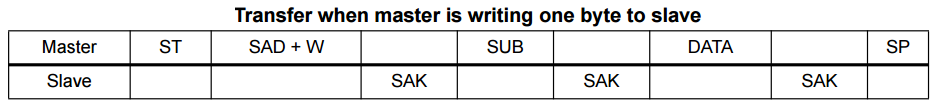
\includegraphics[scale=0.75]{figures/cDesign/Sensor_write_read2.png}
	\caption{På figuren ses metoden for kommunikation mellem slave og master. \citep{STMicroelectronics2016} (Modificeret)}
	\label{Fig:master_slave}
\end{figure}

Det fremgår af figuren, at MCUen skriver en startkode til ICen for at påbegynde kommunikationen mellem master og slave. Herefter skriver masteren én bit til slaven, for at godkende modtagelsen af dette. Dernæst giver masteren en adresse til slaven, som bestemmer hvorfra sensoren skal give data. Når slaven har godkendt dette, skriver masteren til slaven, at den gerne vil læse fra slaven, hvilket tillades og data hentes over på masteren. Afslutningsvist skriver masteren en stop kode til slaven, hvorefter kommunikationen er afbrudt. %For at benytte I$^{2}$C funktionen sættes pin CS\_AG høj, og de fire pins SDO og CS benyttes ikke. Alle pins kan ses på \figref{IC_pins}. Før et signal kan registreres kobles pinnen GND til jord, og på benet VDD skal der leveres mellem 1,9 V og 3,6 V.\fxnote{skriv resten af opsætningen efter at have snakket med John}. \\

Gyroskopet i LSM9DS1 forbruger 4~mA og accelerometeret forbruger 600~$\mu$A under normale betingelser \citep{Jimb02016}\fxnote{hvor Vdd er forsynet med 2,2~V og temperaturen er 25 grader}. For at sikre en høj batterilevetid, er det væsentligt at gyroskopet er aktiveret så kort tid som muligt. Det fremgår af databladet for ICen, at det er muligt at slukke begge sensorer, at benytte accelerometeret alene eller benytte accelerometeret og gyroskopet sammen. Det er dermed muligt, at benytte accelerometeret og gyroskopet skiftevis. Der kan yderligere spares strøm ved brug af gyroskopet, hvis der vælges en lavere samplerate.\\ % alt efter hvor hurtigt et signal skal samples. 
Gyroskopet har tre forskellige power modes; slukket, low power og normal power. For at gyroskopet kan være i low power, skal outputtet af data være på 14,9~Hz til 119~Hz. Hvis outputsignalet er over dette, vil gyroskopet automatisk gå i normal power. %Ifølge \secref{Sec:krav} skal gyroskopet samples med mindst 60 Hz, hvorfor gyroskopet vælges til en samplingsfrekvens på 119~Hz. Derfor er gyroskopet i stand til at gå i low power mode ved den pågældende samplingsfrekvens. \citep{STMicroelectronics2016}
%Accelerometeret og gyroskopet har 32 åbninger af 16 bit data FIFO til hver af gyroskopets akser, samt 16 bit FIFO til hver af accelerometerets akser. Derved skal data ikke konstant sendes til en enhed og der kan spares strøm. Bufferen kan virke på fem forskellige måder, hvor der er tre overordnede tilstande: Bypass tilstand, FIFO tilstand og kontinuert tilstand, som alle tre er illustreret på \figref{tilstand}. Derudover er der to kombinerede tilstande: kontinuert-til-FIFO tilstand og bypass-til-kontinuert tilstand. \newline
%\begin{figure}[H]
%	\centering
%	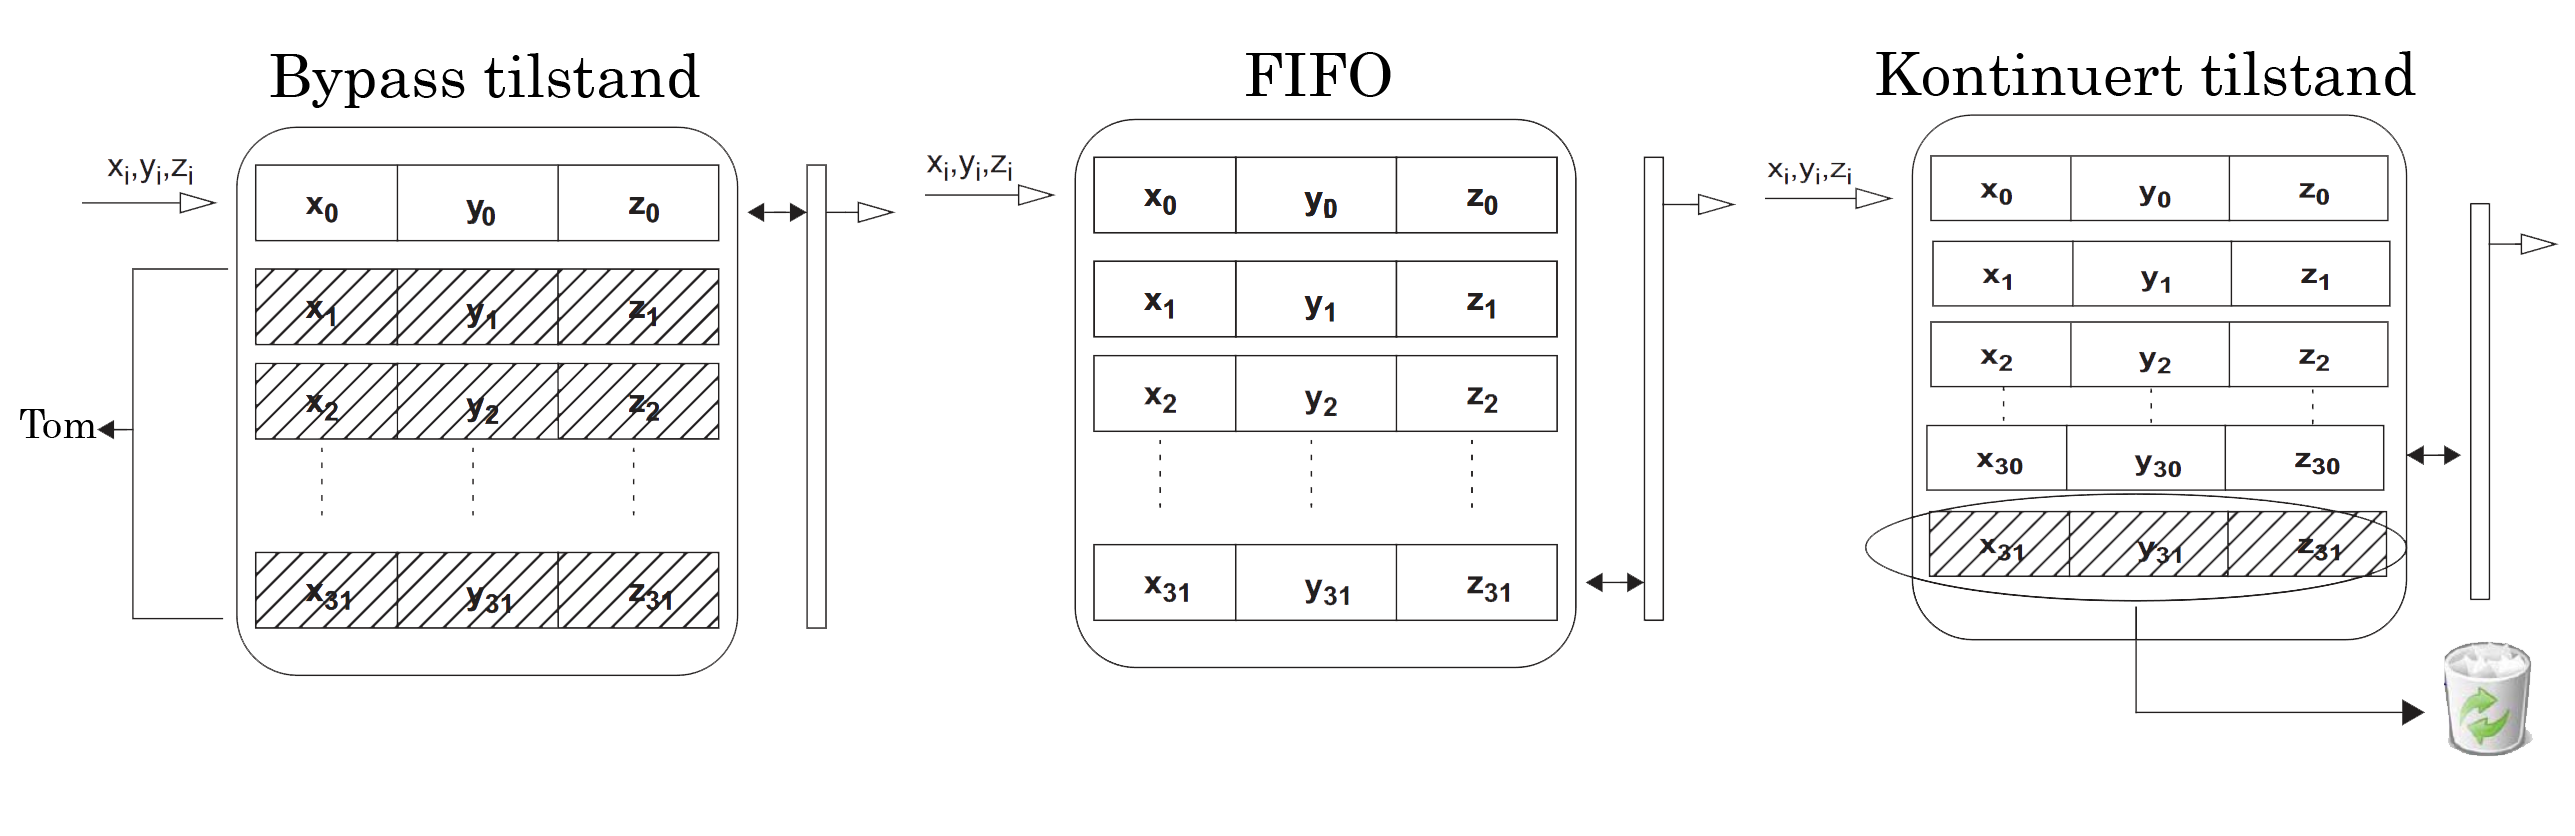
\includegraphics[scale=0.28]{figures/cDesign/LSM9DS1_tilstand.png}
%	\caption{På figuren ses de tre overordnede tilstande IC'en kan opsamle data med.\citep{Jimb02016}}
%	\label{tilstand}
%\end{figure}
%I bypass tilstanden bruges kun den første adresse, som overskrives når ny data er tilgængelig. Denne tilstand benyttes blandt andet til at nulstille FIFO
%FIFO stilstanden bruges til at lagre data i niveauer indtil ny data overskriver det gamle. Det er muligt at gemme data i 32 niveauer, men dette kan tilpasses mindre efter behov. For at gammel data ikke overskrides indsættes et interrupt når FIFO er fyldt, hvormed der ikke lagres ny data. 
%Den kontinuerte tilstand muliggør kontinuert FIFO, hvormed ny data overskriver gammel data. 
%Ved kontinuert-til-FIFO tilstand skifter tilstanden alt efter de bit der modtages i interruptet for accelerometeret og gyroskopet. Hvis der modtages et bit på 1 vil den være i FIFO tilstand, og modtages der et bit på 0, vil den være i kontinuert tilstand. 
%I bypass-til-kontinuert tilstand skiftes der ligeledes mellem bypass og kontinuert tilstand alt efter det modtagne interrups for accelerometeret og gyroskopet. Hvis der modtages et bit på 1, er den i kontinuert tilstand, og modtages der en bit på 0, nulstilles den ved at gå i bypass tilstand. 
\subsection{Implementering}
MCUen kræver en ekstern pull-up modstand tilkoblet for at opsætte I$^{2}$C bussen, hvilket fremgår af \secref{design_lsm}. En ekstern modstand på 4,7~$k\Omega$ forbinder henholdsvis SCL og VDD samt SDA og VDD, hvilket gør I$^{2}$C bussen tilgængelige for dataoverførsel.

I PSoC Programmer indhentes det analoge komponent I2CM. Denne skaber en I$^2$C forbindelse imellem MCUen og ICen samtidig med, at den indstiller MCUen til at være master. %Når PSoC Programmer benyttes til test af sensoren, er der ikke behov for flere komponenter, men hvis dataen skal sendes ind i eksempelvis matlab, kræver det et UART komponent. 
Topdesignet for I2CM modulet konfigureres ydermere til at have sensorens SDA og SCL pins koblet til MCUen på de valgte pins.\\
MCuen skal kunne modtage data fra sensoren, hvilket udførs ved at implementere en algoritme i MCUen. Algoritmen skriver til den hexadresse som er registeradressen dataoutout for accelerometeret og gyroskopet. Således kan MCUen som master skrive til selve accelerometret eller gyroskopet. Der ønskes ydermere, at benytte en samplingsfrekvens på 476~Hz og et arbejdsområde på $\pm$16~g for accelerometeret. Det fremgår af registeret, at der skal skrives til hexadressen 'A8' for at konfigurere accelerometeret til disse indstillinger. \\
Yderligere fremgår det, at hexkoden '79' konfiguerer gyroskopet til de ønskede indstillinger på 2000~dps og en samplingsfrekvens på 119~Hz. \citep{STMicroelectronics2016}


\subsection{Test}
Accelerometeret er indstillet til $\pm$16~g, hvorfor det antages, at den kan opsamle op til $\pm$16 g. Ifølge accelerometerets andet krav i \secref{sec:krav} skal det angive korrekt g-påvirkning med en maks afvigelse på 5\%. Dette testes ved at påvirke sensorens y akse med $\pm$1~g, da denne akse på accelerometret benyttes til detektering af gang og løb, som beskrevet i \secref{bevaegelse}. Det vil i den samlede systemtest, blive testet om accelerometerets signaler klippes. 

ICens accelerometer har en sensitivitet på 0,000732~g per LSB \citep{STMicroelectronics2016}. Outputtet fra sensoren er low byte og high byte, hvilket bliver bitskiftet og derefter adderet i MCUen, hvormed output fra MCUen er i LSB. For at omregne dette output til g skal outputtet ganges med sensitiviteten, hvilket sker i tredje kolonne i \tabref{tab:test_sensor}

Det testes hvilket output y-aksen har, når sensoren er placeret således y-aksen er i horisontal retning. Ved denne placering bør sensoren teoretisk have et output svarende til 0~g. Efterfølgende placeres sensoren med y-aksen i vertikal retning, hvilket teoretisk burde have en påvirkning på $\pm$1~g. Inden målingen testes fladen der måles på med vatterpas, for at sikre, at kun den ønskede akse påvirkedes i vertikal retning. I \tabref{tab:test_sensor} ses resultatet fra testen. 
\begin{table}[H]
	\centering
	\begin{tabular}{cccc} \hline
		\rowcolor[HTML]{C0C0C0} 
		Teoretisk påvirkning {[}g{]} & \begin{tabular}[c]{@{}c@{}} Output fra MCU \\ {[}LSB{]} \end{tabular} & \begin{tabular}[c]{@{}c@{}} Output fra MCU \\ {[}g{]} \end{tabular} & \begin{tabular}[c]{@{}c@{}} Afvigelse \\ {[}\%{]} \end{tabular} \\ \hline
		0 & 19 & 0,014 & 1,4\\ \hline
		+1 & 1368 & 1,003 g & 0,3\\ \hline
		-1  & -1356 & -0,993 g & -0,7\\ \hline
	\end{tabular}%
	\caption{I tabellen ses resultatet fra testen af accelerometerets y-akse. For at omregne MCUens output fra LSB til g påvirkning multipliceres outputtet med accelerometerets sensitivitet.}
	\label{tab:test_sensor}
\end{table}\vspace{-0.2cm}
Det ses i \tabref{tab:test_sensor}, at sensorens accelerometer har en afvigelse på 0,3~\% til 1,4~\%, hvilket overholder en accepteret afvigelse på 5\%, jævnfør \secref{krav:acc}. Det er ydermere antaget, at accelerometeret overholder arbejdsområdet på den indstillede værdi $\pm$16~g, indtil det samlede system giver mulighed for at teste dette. Sensorens accelerometer overholder dermed de opstillede krav og er klar til videre implementering. 

Gyroskopet i ICen har en sensitivitet på 0,070 dps per LSB, når den måler med 2000 dps. Ifølge krav til gyroskopet i \secref{krav:gyro} skal sensoren have et arbejdsområde på mindst 334,69 dps, hvilket overholdes ved valg af 2000 dps. Outputtet fra gyroskopet gives ligeledes i LSB, hvorfor eksempelvis 360 dps, der svarer til én rotation i sekundet, giver et output på 5.142. Det er imidlertid ikke muligt for projektgruppen at teste hvorvidt gyroskopet giver korrekt output, da dette kræver en kontrolleret cirkulær acceleration om en given akse, hvilket kræver udstyr der ikke er i besiddelse.\\
Hvis sådanne udstyr fandtes, havde det været fordelagtigt med en cirkulær plade, hvis omdrejninger skulle være kontrollerbare. Derved kunne den indstilles til for eksempel en omdrejning i sekundet, og i så fald burde gyroskopet måle 360 dps.
%
%
%Accelerometrets sensitivitet ved 16 g målinger: 0,732 mg/LSB
%Hvor LSB er 2*16/2^16 = 0.0078125
%(Man får et output på ca. 1350 fra acc, hvilket giver næsten 1 ganget med 0,732 mg/LSB)
%
%Gyroskopets sensitivitet med 2000 dps målinger: 70 mdps/LSB (17,5 hvis 500)
%Hvor LSB er 2*2000/2^16 = 0.97656
%()